\section{Diskussion}
\label{sec:Diskussion}
Der statistische Fehler der Nullrate ist durch die lange Messzeit sehr gering. Für $\ce{^52 V}$ wurde eine
Halbwertszeit von $T_{\symup{Vanadium}} = (108 \pm 5)\,\unit{\second}$ bestimmt. Der Theoriewert liegt bei
$T_{\symup{Theorie, Vanadium}} = 224,6\,\unit{\second}$ \cite{periodensystem}. Daraus folgt eine Abweichung
von $108\,\%$. Für $\ce{^108 Ag}$ und $\ce{^110 Ag}$ liegen die Theoriewerte bei
$T_{\symup{Theorie, \ce{^108 Ag}}} = 142,2\,\unit{\second}$ und bei
$T_{\symup{Theorie, \ce{^110 Ag}}} = 24,6\,\unit{\second}$ \cite{periodensystem}. Daraus folgen Abweichungen von
$219\,\%$ und $65\,\%$. Die Abweichungen sind sehr groß. Dies lässt sich dadurch erklären, dass für die Messungen
ein großes Messinterval $\Delta t$ verwendet wurde. Ein kleineres Intervall hätte die Messung wesentlich präziser
gemacht. Die Abweichungen für die Halbwertszeiten der Silberpräparate resultieren aus der ungenauen Bestimmung
des Zeitpunkts $t^*$ ab dem der längere Zerfall fast ausschließlich vorkommt.

\section{Anhang}
\label{sec:Anhang}
\begin{figure}
    \centering
    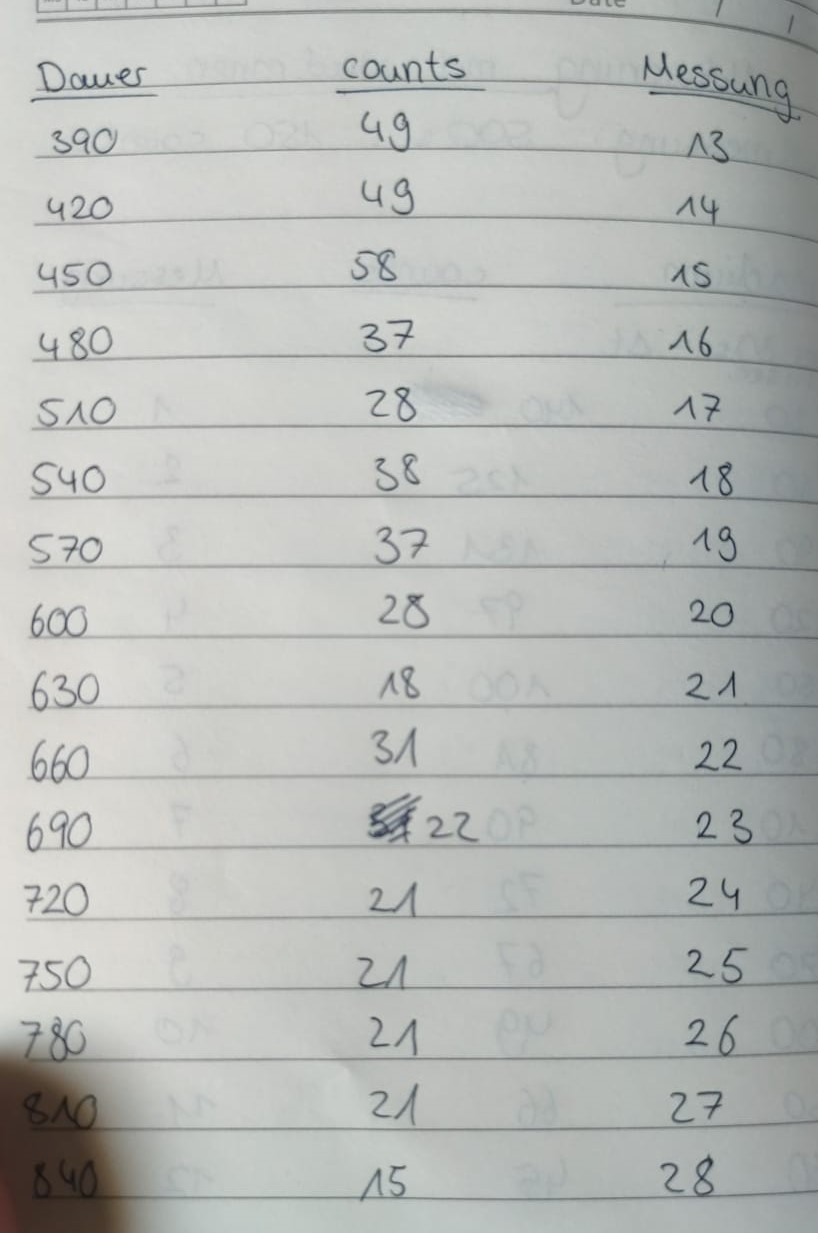
\includegraphics[width=0.7\textwidth]{Bilder/1.jpeg}
    \caption{Messdaten Teil 1.}
    \label{fig:M1}
\end{figure}

\begin{figure}
    \centering
    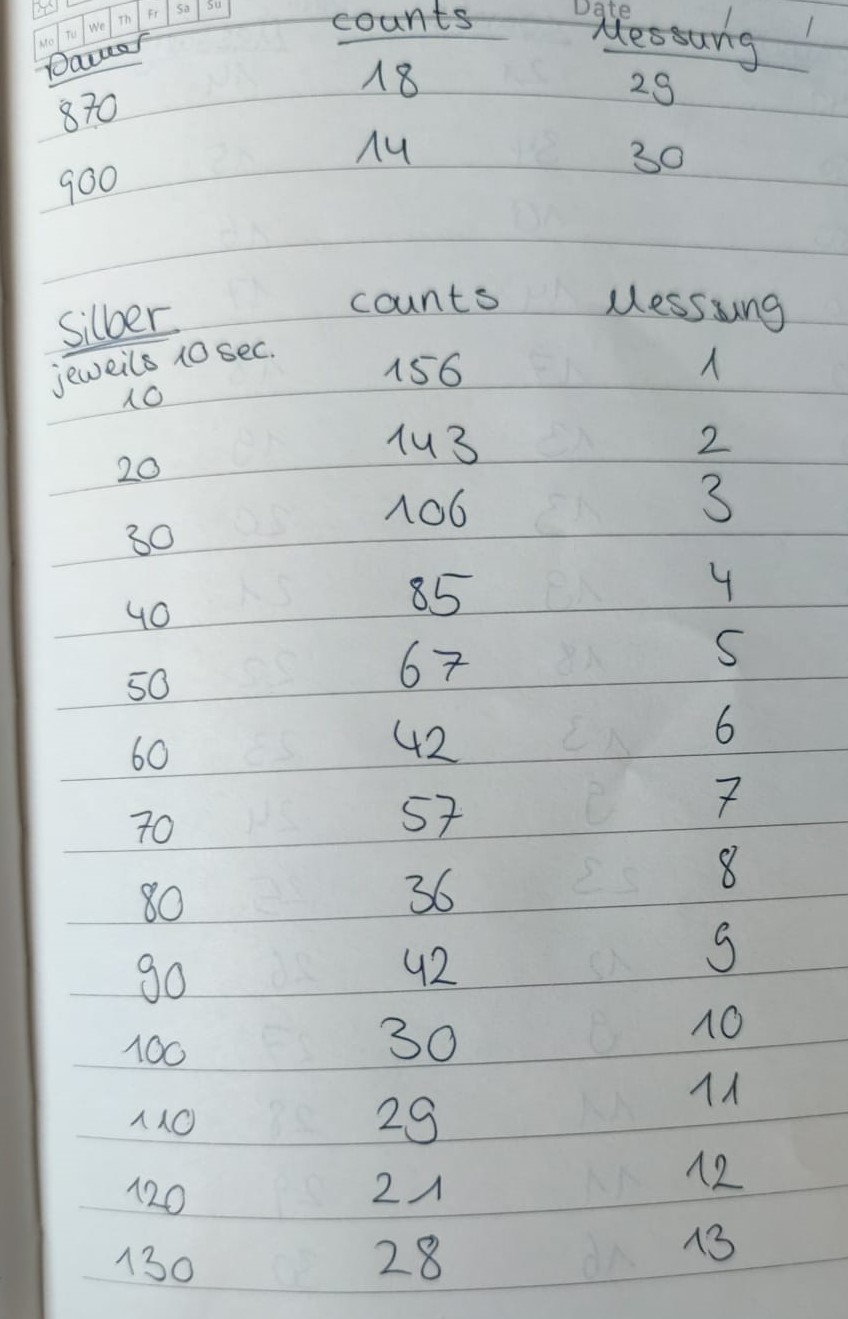
\includegraphics[width=0.7\textwidth]{Bilder/2.jpeg}
    \caption{Messdaten Teil 2.}
    \label{fig:M1}
\end{figure}

\begin{figure}
    \centering
    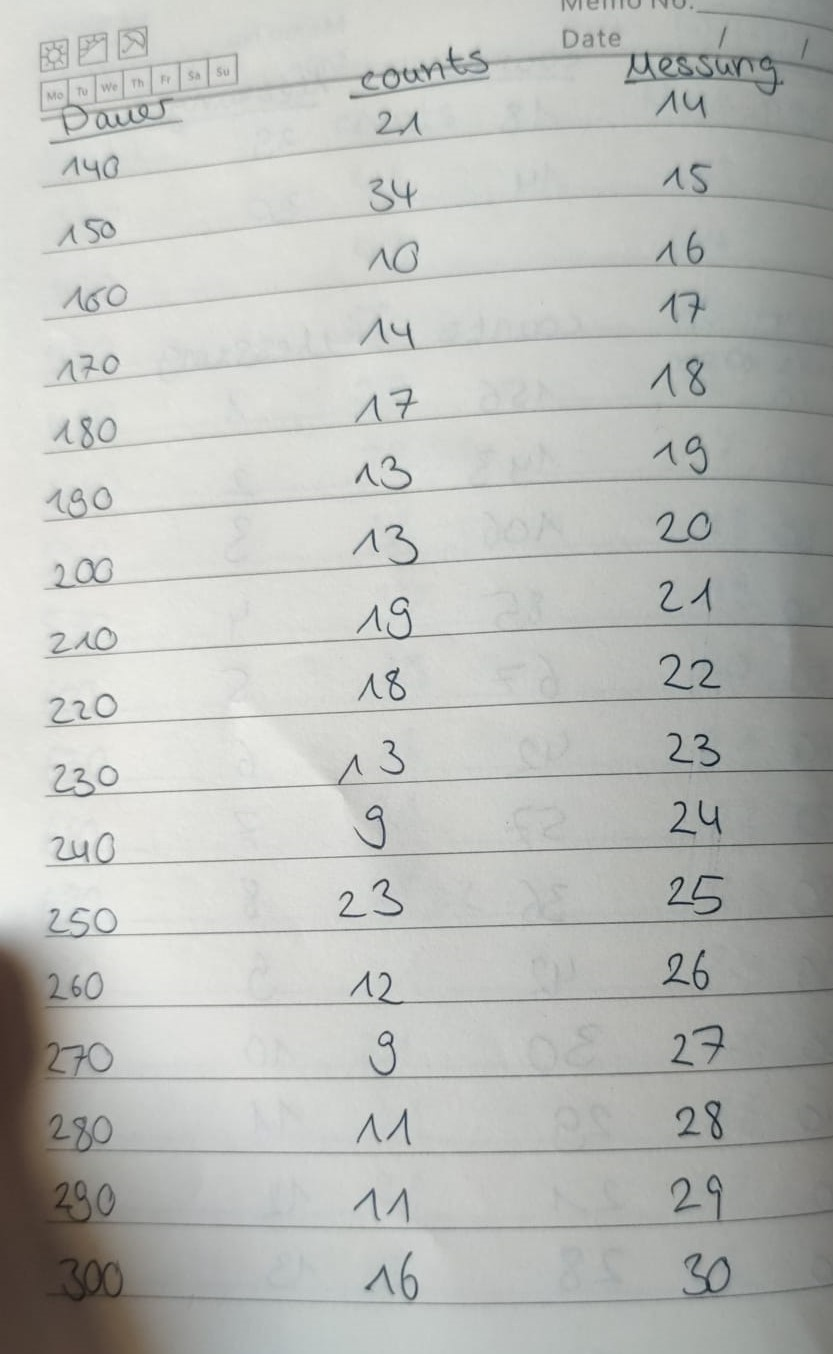
\includegraphics[width=0.7\textwidth]{Bilder/3.jpeg}
    \caption{Messdaten Teil 3.}
    \label{fig:M1}
\end{figure}

\begin{figure}
    \centering
    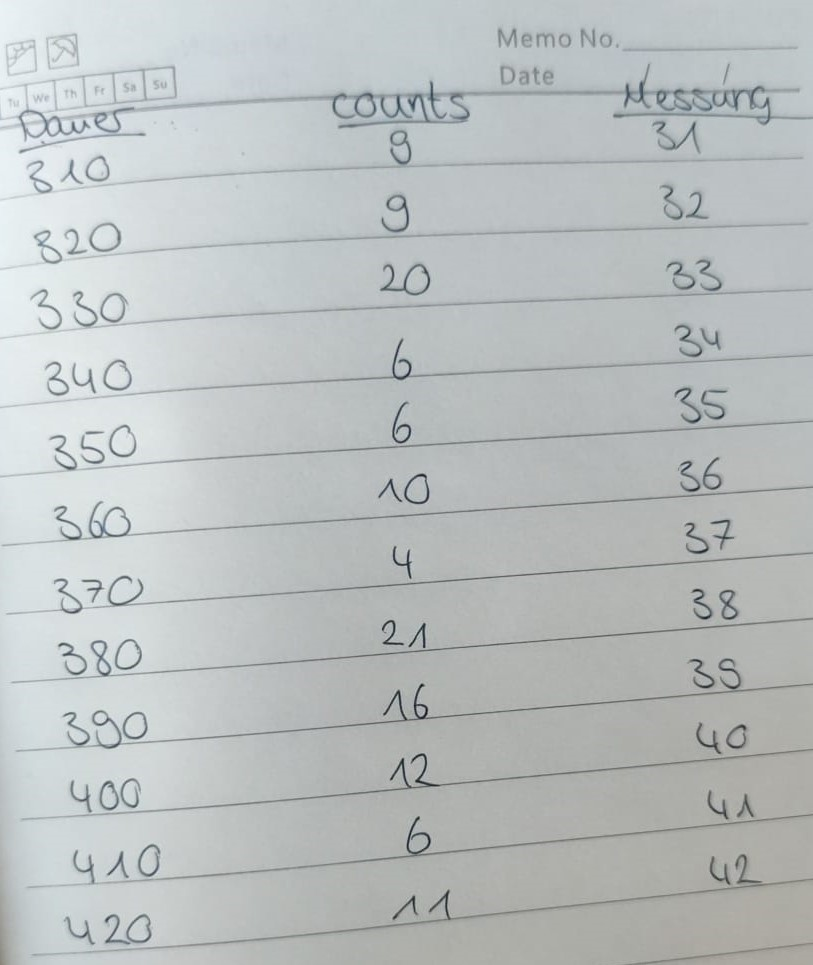
\includegraphics[width=0.7\textwidth]{Bilder/4.jpeg}
    \caption{Messdaten Teil 4.}
    \label{fig:M1}
\end{figure}